\chapter{Appendix A}

This appendix is intended to 

\section{A simple program}

\subsection{Register aliasing}

In order to make writing code simple we used some more mnemonic aliases for the registers, making it simpler to access registers.

\begin{lstlisting}
	CMU .req R4
	GPIO_LED .req R5
	GPIO_btn .req R6
	GPIO .req R7
	EMU .req R8
	
	ldr GPIO_LED, =GPIO_PA_BASE
	ldr GPIO_btn, =GPIO_PC_BASE
	ldr CMU, =CMU_BASE
	ldr EMU, =EMU_BASE
	ldr GPIO, =GPIO_BASE
\end{lstlisting}

\subsection{enabling peripheral clock}

To enable the clock we write to bit 13 of HFPERCLKEN0 by left shifting 1 by 13 and storing it.

\begin{lstlisting}
	mov r2, #1
	lsl r2, r2, #CMU_HFPERCLKEN0_GPIO
	orr r1, r1, r2
	str r1, [CMU, #CMU_HFPERCLKEN0]	
\end{lstlisting}

\subsection{enabling LEDs}

To enable LEDs we write 0x55555555 to GPIO\_PA\_MODEH

\begin{lstlisting}
	mov r1, #0x55
	orr r1, r1, r1, lsl #8
	orr r1, r1, r1, lsl #16
	str r1, [GPIO_LED, #GPIO_MODEH]
\end{lstlisting}

%TODO add a pic from RM to exemplify what writing 0x55555555 actually does.

We set drive strength to high by writing the second bit of GPIO\_PA\_BASE to 1

\begin{lstlisting}
	mov r1, #0x2
	str r1, [GPIO_LED, #GPIO_CTRL]
\end{lstlisting}

\subsection{enabing buttons}

To set pins 0-7 as input we write 0x33333333 to GPIO\_PC\_MODEL

\begin{lstlisting}
  mov r1, #0x33
  orr r1, r1, r1, lsl #8
  orr r1, r1, r1, lsl #16
  str r1, [GPIO_btn, #GPIO_MODEL]
\end{lstlisting}

Enabling button pull-up

\begin{lstlisting}
  mov r1, #0xff
  str r1, [GPIO_btn, #GPIO_DOUT]
\end{lstlisting}

The polling loop continuously reads which buttons are pressed from GPIO\_PC\_ and writes them to 

\section{Interrupt based implementation}

Setting port C as interrupt source by writing 0x22222222 to GPIO\_EXTIPSELL

\begin{lstlisting}
	ldr r1, =0x22222222
	str r1, [GPIO, #GPIO_EXTIPSELL]
\end{lstlisting}

Set 1->0 and 0->1 to trigger interrupt by writing 0xFF to GPIO\_EXTIPFALL and EXTIPRISE

\begin{lstlisting}
	// Set interrupt on 1->0
	ldr r1, =0x0ff
	str r1, [GPIO, #GPIO_EXTIFALL]

	// Set interrupt on 0->1
	str r1, [GPIO, #GPIO_EXTIRISE]
\end{lstlisting}

Activating interrupt generation by writing 0x6 to ISER0

\begin{lstlisting}
	ldr r1, =ISER0
	ldr r2, =0x802
	str r2, [r1]
\end{lstlisting}

\section{Handling interrupts}

To handle gpio interrupts the handler reads from GPIO\_IF interrupt flag register, and stores it in the GPIO\_IFC, interrupt flag cleared register.

\begin{lstlisting}
	ldr r1, [GPIO, #GPIO_IF]	
	str r1, [GPIO, #GPIO_IFC]	
\end{lstlisting}

%TODO, something about the gpio handler

\section{Efficient interrupts}

Enabling deep sleep on exiting interrupt handler by writing 0x6 to SCR, the system control register 

\begin{lstlisting}
	ldr r1, =SCR
	mov r2, #6
	str r2, [r1]	
\end{lstlisting}

Waiting for interrupt

\begin{lstlisting}
program_loop:
 	wfi
	b program_loop  	
\end{lstlisting}

The loop isnt strictly necessary as the processor wont execute anything after hitting the wfi instruction.

\section{Further improvements}

To disable SRAM blocks we write 0x7 to the EMU\_MEMCTRL to set all POWERDOWN bits to 1.

\begin{lstlisting}
	mov r1, #0x7
	str r1, [EMU, #EMU_MEM_CTRL]
\end{lstlisting}

To reflect the changed memory layout we change the linker script, specifically, ram LENGTH is now 32kb

\begin{lstlisting}
MEMORY
{
  rom (rx) : ORIGIN = 0x00000000, LENGTH = 1048576
  ram (rwx) : ORIGIN = 0x20000000, LENGTH = 32768
}
\end{lstlisting}

To disable the low frequency peripheral clocks LFACLK and LFBCLK we write 0x0 to CMU\_LFCLKSEL

\begin{lstlisting}
	mov r1, #0x0
	str r1, [CMU, #CMU_LFCLKSEL]
\end{lstlisting}

\begin{figure}[ht]
 \centering
 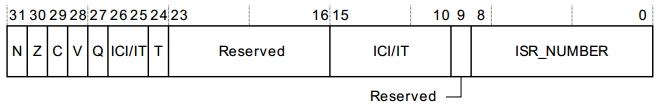
\includegraphics[width=\textwidth]{images/psrMap.png}
 \caption{PSR bitmap}
 \label{fig:psrMap}
\end{figure}